\documentclass[12pt]{article}

\usepackage[utf8]{inputenc}
\usepackage[T1]{fontenc}
\usepackage[top=2cm, bottom=2cm, left=2cm, right=2cm]{geometry}
\usepackage{url}
\usepackage{graphicx}
\hbadness=99999
\title{TD4 - InfoEmb}
\author{Jérôme Skoda, Joaquim Lefranc}
\date{Novembre 2017}

\begin{document}
\fontfamily{cmr}
\maketitle

\section{Estimations}
\textbf{Initiale :} 4h (Pas le choix il faut le rendre dans 4h) \newline
\textbf{Réel :} 7h: (4h + 3h d'extra)

\section{Etapes pour la création/destruction}

	\subsection{Quel outil pour quelle mesure?}
		Et bien il faut mesurer le total, donc la ramette, puis le diviser par le nombre de feuilles dans la ramette. C'est le même principe avec le temps dans le tp. On peut mesurer un gros bloc d'opérations puis diviser le total par le nombre d'opérations dans le bloc.

	\subsection{(Optionnel) Fonctions de mesure de temps sous linux}

	gettimeofday(): C'est un appel system, il retourne le nombre de secondes écoulées depuis le 01/01/1970. Elle donne aussi les microsecondes. La précision est environ de 0,5ms sur Debian (Comme vu dans vos cours). (Temp mural)
	\newline

	time\_t time : Elle vient de la librairie time.h, le point de départ est 01/01/1970. (Temp mural)
	\newline

	clock\_gettime : Elle vient de la librairie time.h, elle peut mesurer le temps de différentes façons, elle retourne un résultat en secondes ou nanosecondes.
	\newline

	clock : Elle vient de la librairie time.h, temps de départ : lancement du processus (Mesure du temps CPU)
	\newline
	times : C'est une app system : Page (1) du man.
	\newline


	\subsection{Mesure d'opérations en C : résultat des deux mesures}

		\textbf{Processus}\newline
		\textit{Source: tempsExecution/processus.c} \newline
		Point initial de mesure du temps: Avant la boucle de fork \newline
		Point final de mesure du temps: Après la boucle de fork \newline
		\newline

		Les mesures prennent le temps de création d'un fork ainsi que l'incrémentation
		de la variable n\_processus. La mesure du temps d'incrementation parasite
		légèrement la mesure mais il s'agit surement de la solution la plus
		compréhensible et simple à mettre en oeuvre.\newline
		\newline

		\textbf{Thread}\newline
		\textit{Source: tempsExecution/thread.c}\newline
		Point initial de mesure du temps: Avant la boucle de pthread\_create\newline
		Point final de mesure du temps: Après la boucle de pthread\_create\newline
		\newline
		Comme pour la messure des processus, l'incrémentation de la variable
		n\_thread parasite la mesure.\newline

		Résultat obtenu

		Chacun des résultat suivant sont produit avec "taskset -c 0" pour avoir
		une exécution sur un seul coeur.

		\begin{center}
		  \begin{tabular}{ | c | c | c | }
				\hline
					&	Desktop      &    Laptop \\
				\hline
					processus & 53.939709 ms  &     86.157382 ms \\
				\hline
					thread    & 12.604273 ms  &      24.614902 ms \\
				\hline
			\end{tabular}
		\end{center}

		Desktop: CPU: i7 4790K @ 4.3GHz 4 cores 8 threads RAM: 16Go @ 1 600MHz
		Laptop: CPU: i5-2430M @ 2.40GHz 2 cores 4 threads RAM: 32Go @ 1 600MHz

	\subsection{Répétez votre mesure. Plusieurs fois. Le résultat obtenu est-il constant? Quelles méthodes statistiques devraient être utilisées pour « publier » des résultats ?}

		Le résultat n'est pas contant et il est fort probable que les résultat suivent
		une loi normale, utiliser une medianne, l'écart type ou la variance semble plus approprié.
		\newline

	\subsection{Phénomènes et facteurs qui peuvent influencer la mesure}

		Les caractéritique physique d'une machine peuvent faire varier énormement les
		mesures (nombre de coeurs, fréquence etc) ainsi que l'état de la machine à
		l'instant de l'éxecution (nombre de processus actif).
		Il n'est pas possible de fournir un temps minimum ni même un temps maximum,
		cependant il est possible d'établir une ordre de grandeur.
		La création d'un thread est plus rapide de 3 à 5 fois que la création d'un
		processus.\newline

		Créer un thread prendre dans l'ordre de la dizaine de microseconde. \newline
		Créer un processus prend dans l'ordre de la cinquantaine de microseconde.\newline

\section{Changement de contexte}

Source: tempsContext/processus.c et tempsContext/thread.c

\begin{center}
	\begin{tabular}{ | c | c | c | }
		\hline
			&	Desktop      &    Laptop \\
		\hline
			processus & 1.187886 ms &  2.895871 ms \\
		\hline
			thread    & 0.911997 ms &  3.544407 ms \\
		\hline
	\end{tabular}
\end{center}

Desktop: CPU: i7 4790K @ 4.3GHz 4 cores 8 threads RAM: 16Go @ 1 600MHz
Laptop: CPU: i5-2430M @ 2.40GHz 2 cores 4 threads RAM: 32Go @ 1 600MHz

Pour faire l'ordonnancement, nous avons utilisé deux sémaphore: un est ouvert
et l'autre bloqué à l'état initial. Chacun des processus ou thread attendent
chacun l'ouverture d'un sémaphore et ouvre l'autre. De cette manière on obtien
l'ordonnancement P1 P2 P1 P2 etc.

Les résultat peuvent varier en fonction de de sémaphore utilisé exemple
dans thread.c avec des sémaphore partagé, le changement de contexte est plus
long.


Source: expliciteFIFO/processus.c et expliciteFIFO/thread.c et  impliciteFIFO/processus.c et impliciteFIFO/thread.c  

Le changement de contexte implicite et explicite, on remarque que les thread sont plus rapide.

Voici un graph sur basé sur 1000 échantillon de moyenne. 
Le maximum de chaque courbe représente le résultat qui a statistiquement plus de chance de tomber.

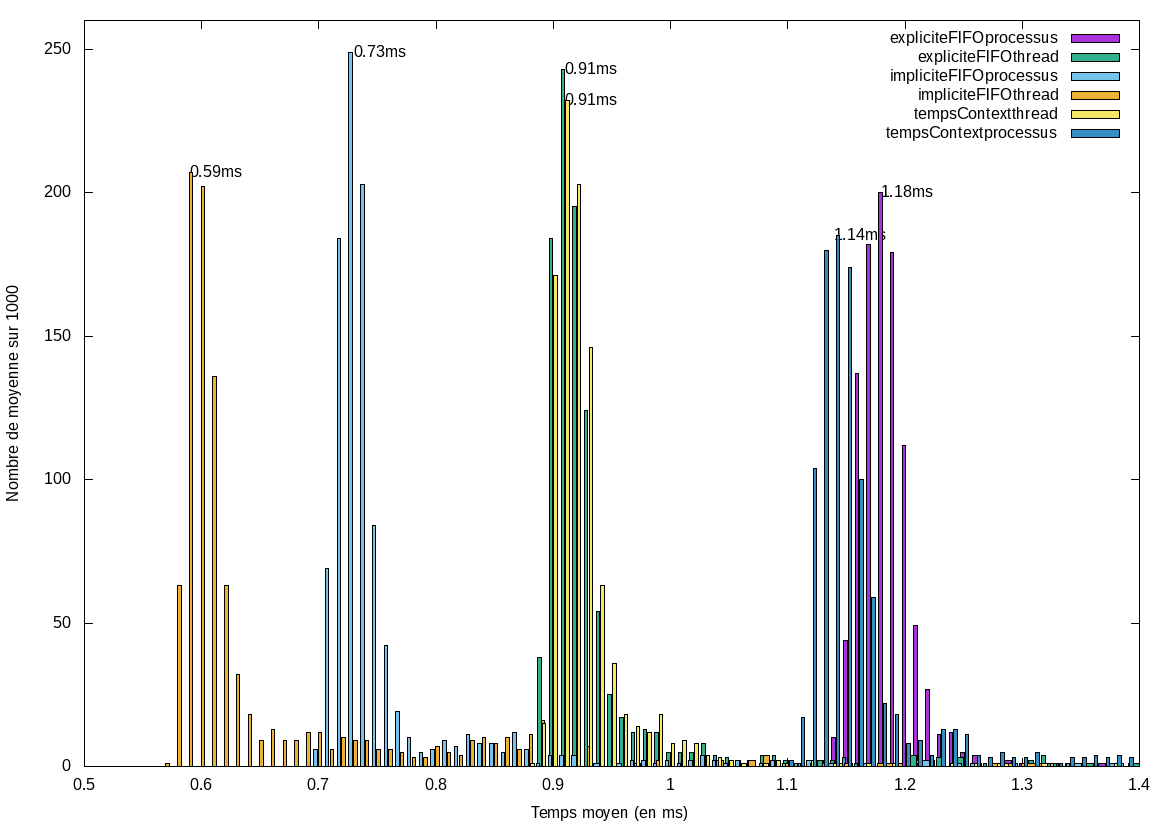
\includegraphics[width=\linewidth]{graph.png}.

\section{Comparaison avec d'autres résultats de TP}

Les différences peuvent venir du type de processeur, de sa charge actuelle (nombre d'applications éxécutées).
De plus certain processeurs diminiuent leurs vitesse de fonctionnement ce qui peut influer sur le résultat.
Cependant nos résultats sont cohérents avec ceux d'autres groupes, les ordres de grandeurs sont respectés.

\section{Outils de « benchmarking »}
La commande ./lat\_proc -N 1000 fork nous donne une granularité de 62 microsecondes. \newline

La personne chargé de cette partie est parti en voyage aux Bahamas.

\end{document}
